% Created by tikzDevice version 0.12.3.1 on 2021-07-06 14:19:28
% !TEX encoding = UTF-8 Unicode
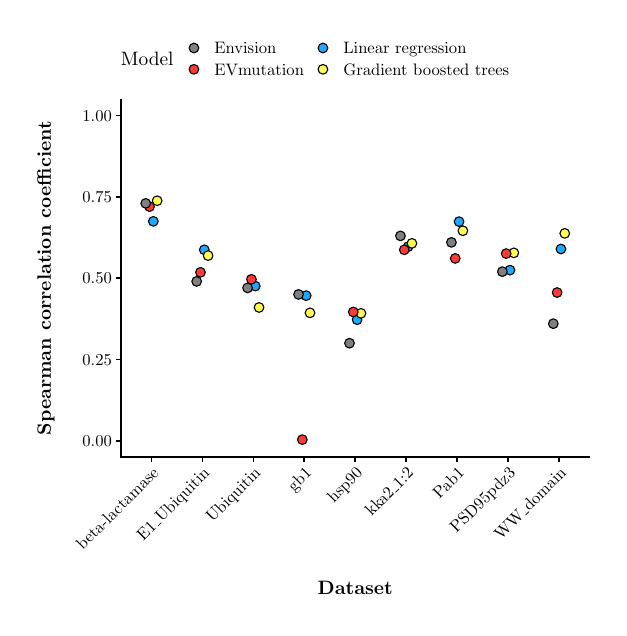
\begin{tikzpicture}[x=1pt,y=1pt]
\definecolor{fillColor}{RGB}{255,255,255}
\path[use as bounding box,fill=fillColor,fill opacity=0.00] (0,0) rectangle (206.56,209.59);
\begin{scope}
\path[clip] ( 33.67, 54.47) rectangle (203.06,183.69);
\definecolor{drawColor}{RGB}{0,0,0}
\definecolor{fillColor}{RGB}{31,168,255}

\path[draw=drawColor,line width= 0.4pt,line join=round,line cap=round,fill=fillColor] ( 45.41,139.61) circle (  1.75);
\definecolor{fillColor}{RGB}{255,253,82}

\path[draw=drawColor,line width= 0.4pt,line join=round,line cap=round,fill=fillColor] ( 46.79,147.05) circle (  1.75);
\definecolor{fillColor}{RGB}{255,56,56}

\path[draw=drawColor,line width= 0.4pt,line join=round,line cap=round,fill=fillColor] ( 44.03,144.92) circle (  1.75);
\definecolor{fillColor}{RGB}{31,168,255}

\path[draw=drawColor,line width= 0.4pt,line join=round,line cap=round,fill=fillColor] ( 63.82,129.32) circle (  1.75);
\definecolor{fillColor}{RGB}{255,253,82}

\path[draw=drawColor,line width= 0.4pt,line join=round,line cap=round,fill=fillColor] ( 65.20,127.22) circle (  1.75);
\definecolor{fillColor}{RGB}{255,56,56}

\path[draw=drawColor,line width= 0.4pt,line join=round,line cap=round,fill=fillColor] ( 62.44,121.18) circle (  1.75);
\definecolor{fillColor}{RGB}{31,168,255}

\path[draw=drawColor,line width= 0.4pt,line join=round,line cap=round,fill=fillColor] ( 82.23,116.21) circle (  1.75);
\definecolor{fillColor}{RGB}{255,253,82}

\path[draw=drawColor,line width= 0.4pt,line join=round,line cap=round,fill=fillColor] ( 83.61,108.49) circle (  1.75);
\definecolor{fillColor}{RGB}{255,56,56}

\path[draw=drawColor,line width= 0.4pt,line join=round,line cap=round,fill=fillColor] ( 80.85,118.66) circle (  1.75);
\definecolor{fillColor}{RGB}{31,168,255}

\path[draw=drawColor,line width= 0.4pt,line join=round,line cap=round,fill=fillColor] (100.64,112.76) circle (  1.75);
\definecolor{fillColor}{RGB}{255,253,82}

\path[draw=drawColor,line width= 0.4pt,line join=round,line cap=round,fill=fillColor] (102.02,106.54) circle (  1.75);
\definecolor{fillColor}{RGB}{255,56,56}

\path[draw=drawColor,line width= 0.4pt,line join=round,line cap=round,fill=fillColor] ( 99.26, 60.73) circle (  1.75);
\definecolor{fillColor}{RGB}{31,168,255}

\path[draw=drawColor,line width= 0.4pt,line join=round,line cap=round,fill=fillColor] (119.05,104.06) circle (  1.75);
\definecolor{fillColor}{RGB}{255,253,82}

\path[draw=drawColor,line width= 0.4pt,line join=round,line cap=round,fill=fillColor] (120.44,106.36) circle (  1.75);
\definecolor{fillColor}{RGB}{255,56,56}

\path[draw=drawColor,line width= 0.4pt,line join=round,line cap=round,fill=fillColor] (117.67,106.86) circle (  1.75);
\definecolor{fillColor}{RGB}{31,168,255}

\path[draw=drawColor,line width= 0.4pt,line join=round,line cap=round,fill=fillColor] (137.47,130.46) circle (  1.75);
\definecolor{fillColor}{RGB}{255,253,82}

\path[draw=drawColor,line width= 0.4pt,line join=round,line cap=round,fill=fillColor] (138.85,131.65) circle (  1.75);
\definecolor{fillColor}{RGB}{255,56,56}

\path[draw=drawColor,line width= 0.4pt,line join=round,line cap=round,fill=fillColor] (136.09,129.31) circle (  1.75);
\definecolor{fillColor}{RGB}{31,168,255}

\path[draw=drawColor,line width= 0.4pt,line join=round,line cap=round,fill=fillColor] (155.88,139.50) circle (  1.75);
\definecolor{fillColor}{RGB}{255,253,82}

\path[draw=drawColor,line width= 0.4pt,line join=round,line cap=round,fill=fillColor] (157.26,136.21) circle (  1.75);
\definecolor{fillColor}{RGB}{255,56,56}

\path[draw=drawColor,line width= 0.4pt,line join=round,line cap=round,fill=fillColor] (154.50,126.21) circle (  1.75);
\definecolor{fillColor}{RGB}{31,168,255}

\path[draw=drawColor,line width= 0.4pt,line join=round,line cap=round,fill=fillColor] (174.29,121.97) circle (  1.75);
\definecolor{fillColor}{RGB}{255,253,82}

\path[draw=drawColor,line width= 0.4pt,line join=round,line cap=round,fill=fillColor] (175.67,128.22) circle (  1.75);
\definecolor{fillColor}{RGB}{255,56,56}

\path[draw=drawColor,line width= 0.4pt,line join=round,line cap=round,fill=fillColor] (172.91,127.95) circle (  1.75);
\definecolor{fillColor}{RGB}{31,168,255}

\path[draw=drawColor,line width= 0.4pt,line join=round,line cap=round,fill=fillColor] (192.70,129.62) circle (  1.75);
\definecolor{fillColor}{RGB}{255,253,82}

\path[draw=drawColor,line width= 0.4pt,line join=round,line cap=round,fill=fillColor] (194.08,135.26) circle (  1.75);
\definecolor{fillColor}{RGB}{255,56,56}

\path[draw=drawColor,line width= 0.4pt,line join=round,line cap=round,fill=fillColor] (191.32,113.88) circle (  1.75);
\definecolor{fillColor}{RGB}{128,128,128}

\path[draw=drawColor,line width= 0.4pt,line join=round,line cap=round,fill=fillColor] ( 42.65,146.10) circle (  1.75);

\path[draw=drawColor,line width= 0.4pt,line join=round,line cap=round,fill=fillColor] (153.12,132.00) circle (  1.75);

\path[draw=drawColor,line width= 0.4pt,line join=round,line cap=round,fill=fillColor] ( 61.06,117.90) circle (  1.75);

\path[draw=drawColor,line width= 0.4pt,line join=round,line cap=round,fill=fillColor] (134.70,134.35) circle (  1.75);

\path[draw=drawColor,line width= 0.4pt,line join=round,line cap=round,fill=fillColor] (171.53,121.43) circle (  1.75);

\path[draw=drawColor,line width= 0.4pt,line join=round,line cap=round,fill=fillColor] (189.94,102.63) circle (  1.75);

\path[draw=drawColor,line width= 0.4pt,line join=round,line cap=round,fill=fillColor] ( 79.47,115.55) circle (  1.75);

\path[draw=drawColor,line width= 0.4pt,line join=round,line cap=round,fill=fillColor] ( 97.88,113.20) circle (  1.75);

\path[draw=drawColor,line width= 0.4pt,line join=round,line cap=round,fill=fillColor] (116.29, 95.58) circle (  1.75);
\end{scope}
\begin{scope}
\path[clip] (  0.00,  0.00) rectangle (206.56,209.59);
\definecolor{drawColor}{RGB}{0,0,0}

\path[draw=drawColor,line width= 0.6pt,line join=round,line cap=rect] ( 33.67, 54.47) --
	( 33.67,183.69);
\end{scope}
\begin{scope}
\path[clip] (  0.00,  0.00) rectangle (206.56,209.59);
\definecolor{drawColor}{RGB}{0,0,0}

\node[text=drawColor,anchor=base east,inner sep=0pt, outer sep=0pt, scale=  0.60] at ( 30.42, 58.28) {0.00};

\node[text=drawColor,anchor=base east,inner sep=0pt, outer sep=0pt, scale=  0.60] at ( 30.42, 87.64) {0.25};

\node[text=drawColor,anchor=base east,inner sep=0pt, outer sep=0pt, scale=  0.60] at ( 30.42,117.01) {0.50};

\node[text=drawColor,anchor=base east,inner sep=0pt, outer sep=0pt, scale=  0.60] at ( 30.42,146.38) {0.75};

\node[text=drawColor,anchor=base east,inner sep=0pt, outer sep=0pt, scale=  0.60] at ( 30.42,175.75) {1.00};
\end{scope}
\begin{scope}
\path[clip] (  0.00,  0.00) rectangle (206.56,209.59);
\definecolor{drawColor}{RGB}{0,0,0}

\path[draw=drawColor,line width= 0.6pt,line join=round] ( 31.92, 60.34) --
	( 33.67, 60.34);

\path[draw=drawColor,line width= 0.6pt,line join=round] ( 31.92, 89.71) --
	( 33.67, 89.71);

\path[draw=drawColor,line width= 0.6pt,line join=round] ( 31.92,119.08) --
	( 33.67,119.08);

\path[draw=drawColor,line width= 0.6pt,line join=round] ( 31.92,148.45) --
	( 33.67,148.45);

\path[draw=drawColor,line width= 0.6pt,line join=round] ( 31.92,177.81) --
	( 33.67,177.81);
\end{scope}
\begin{scope}
\path[clip] (  0.00,  0.00) rectangle (206.56,209.59);
\definecolor{drawColor}{RGB}{0,0,0}

\path[draw=drawColor,line width= 0.6pt,line join=round,line cap=rect] ( 33.67, 54.47) --
	(203.06, 54.47);
\end{scope}
\begin{scope}
\path[clip] (  0.00,  0.00) rectangle (206.56,209.59);
\definecolor{drawColor}{RGB}{0,0,0}

\path[draw=drawColor,line width= 0.6pt,line join=round] ( 44.72, 52.72) --
	( 44.72, 54.47);

\path[draw=drawColor,line width= 0.6pt,line join=round] ( 63.13, 52.72) --
	( 63.13, 54.47);

\path[draw=drawColor,line width= 0.6pt,line join=round] ( 81.54, 52.72) --
	( 81.54, 54.47);

\path[draw=drawColor,line width= 0.6pt,line join=round] ( 99.95, 52.72) --
	( 99.95, 54.47);

\path[draw=drawColor,line width= 0.6pt,line join=round] (118.36, 52.72) --
	(118.36, 54.47);

\path[draw=drawColor,line width= 0.6pt,line join=round] (136.78, 52.72) --
	(136.78, 54.47);

\path[draw=drawColor,line width= 0.6pt,line join=round] (155.19, 52.72) --
	(155.19, 54.47);

\path[draw=drawColor,line width= 0.6pt,line join=round] (173.60, 52.72) --
	(173.60, 54.47);

\path[draw=drawColor,line width= 0.6pt,line join=round] (192.01, 52.72) --
	(192.01, 54.47);
\end{scope}
\begin{scope}
\path[clip] (  0.00,  0.00) rectangle (206.56,209.59);
\definecolor{drawColor}{RGB}{0,0,0}

\node[text=drawColor,rotate= 45.00,anchor=base east,inner sep=0pt, outer sep=0pt, scale=  0.60] at ( 47.64, 48.30) {beta-lactamase};

\node[text=drawColor,rotate= 45.00,anchor=base east,inner sep=0pt, outer sep=0pt, scale=  0.60] at ( 66.05, 48.30) {E1\_Ubiquitin};

\node[text=drawColor,rotate= 45.00,anchor=base east,inner sep=0pt, outer sep=0pt, scale=  0.60] at ( 84.46, 48.30) {Ubiquitin};

\node[text=drawColor,rotate= 45.00,anchor=base east,inner sep=0pt, outer sep=0pt, scale=  0.60] at (102.88, 48.30) {gb1};

\node[text=drawColor,rotate= 45.00,anchor=base east,inner sep=0pt, outer sep=0pt, scale=  0.60] at (121.29, 48.30) {hsp90};

\node[text=drawColor,rotate= 45.00,anchor=base east,inner sep=0pt, outer sep=0pt, scale=  0.60] at (139.70, 48.30) {kka2\_1:2};

\node[text=drawColor,rotate= 45.00,anchor=base east,inner sep=0pt, outer sep=0pt, scale=  0.60] at (158.11, 48.30) {Pab1};

\node[text=drawColor,rotate= 45.00,anchor=base east,inner sep=0pt, outer sep=0pt, scale=  0.60] at (176.52, 48.30) {PSD95pdz3};

\node[text=drawColor,rotate= 45.00,anchor=base east,inner sep=0pt, outer sep=0pt, scale=  0.60] at (194.93, 48.30) {WW\_domain};
\end{scope}
\begin{scope}
\path[clip] (  0.00,  0.00) rectangle (206.56,209.59);
\definecolor{drawColor}{RGB}{0,0,0}

\node[text=drawColor,anchor=base,inner sep=0pt, outer sep=0pt, scale=  0.70] at (118.36,  4.86) {\bfseries Dataset};
\end{scope}
\begin{scope}
\path[clip] (  0.00,  0.00) rectangle (206.56,209.59);
\definecolor{drawColor}{RGB}{0,0,0}

\node[text=drawColor,rotate= 90.00,anchor=base,inner sep=0pt, outer sep=0pt, scale=  0.70] at (  8.39,119.08) {\bfseries Spearman correlation coefficient};
\end{scope}
\begin{scope}
\path[clip] (  0.00,  0.00) rectangle (206.56,209.59);
\definecolor{drawColor}{RGB}{0,0,0}

\node[text=drawColor,anchor=base west,inner sep=0pt, outer sep=0pt, scale=  0.70] at ( 33.67,195.97) {Model};
\end{scope}
\begin{scope}
\path[clip] (  0.00,  0.00) rectangle (206.56,209.59);
\definecolor{drawColor}{RGB}{0,0,0}
\definecolor{fillColor}{RGB}{128,128,128}

\path[draw=drawColor,line width= 0.4pt,line join=round,line cap=round,fill=fillColor] ( 60.08,202.24) circle (  1.75);
\end{scope}
\begin{scope}
\path[clip] (  0.00,  0.00) rectangle (206.56,209.59);
\definecolor{drawColor}{RGB}{0,0,0}
\definecolor{fillColor}{RGB}{255,56,56}

\path[draw=drawColor,line width= 0.4pt,line join=round,line cap=round,fill=fillColor] ( 60.08,194.54) circle (  1.75);
\end{scope}
\begin{scope}
\path[clip] (  0.00,  0.00) rectangle (206.56,209.59);
\definecolor{drawColor}{RGB}{0,0,0}
\definecolor{fillColor}{RGB}{31,168,255}

\path[draw=drawColor,line width= 0.4pt,line join=round,line cap=round,fill=fillColor] (106.69,202.24) circle (  1.75);
\end{scope}
\begin{scope}
\path[clip] (  0.00,  0.00) rectangle (206.56,209.59);
\definecolor{drawColor}{RGB}{0,0,0}
\definecolor{fillColor}{RGB}{255,253,82}

\path[draw=drawColor,line width= 0.4pt,line join=round,line cap=round,fill=fillColor] (106.69,194.54) circle (  1.75);
\end{scope}
\begin{scope}
\path[clip] (  0.00,  0.00) rectangle (206.56,209.59);
\definecolor{drawColor}{RGB}{0,0,0}

\node[text=drawColor,anchor=base west,inner sep=0pt, outer sep=0pt, scale=  0.60] at ( 67.43,200.17) {Envision};
\end{scope}
\begin{scope}
\path[clip] (  0.00,  0.00) rectangle (206.56,209.59);
\definecolor{drawColor}{RGB}{0,0,0}

\node[text=drawColor,anchor=base west,inner sep=0pt, outer sep=0pt, scale=  0.60] at ( 67.43,192.47) {EVmutation};
\end{scope}
\begin{scope}
\path[clip] (  0.00,  0.00) rectangle (206.56,209.59);
\definecolor{drawColor}{RGB}{0,0,0}

\node[text=drawColor,anchor=base west,inner sep=0pt, outer sep=0pt, scale=  0.60] at (114.04,200.17) {Linear regression};
\end{scope}
\begin{scope}
\path[clip] (  0.00,  0.00) rectangle (206.56,209.59);
\definecolor{drawColor}{RGB}{0,0,0}

\node[text=drawColor,anchor=base west,inner sep=0pt, outer sep=0pt, scale=  0.60] at (114.04,192.47) {Gradient boosted trees};
\end{scope}
\end{tikzpicture}
